\documentclass[11pt]{article}

% Math
\usepackage{amsmath, amssymb, amsfonts, mathtools}

% Page layout
\usepackage[margin=1in]{geometry}

% Optional useful packages
\usepackage{physics}      % \bra, \ket, \dv, \pdv, etc.
\usepackage{bm}           % bold math symbols
\usepackage{bbm}
\usepackage{enumitem}     % better lists
\usepackage{graphicx}     % Required for inserting images
\usepackage{subcaption}   % Required for the subfigure environment
\usepackage{hyperref}     % links
\hypersetup{
    colorlinks=true,       % false: boxed links; true: colored links
    linkcolor=blue,        % color of internal links (sections, pages, etc.)
    citecolor=green,       % color of citation links to bibliography
    % filecolor=magenta,     % color of file links
    urlcolor=blue,         % color of external website links
    % allcolors=blue       % uncomment this if you want ALL links to use one color
}

\title{Weekly Update}
\author{Reza Asakereh}
\date{Last Update: \today}

\begin{document}

\maketitle

\section{Main Findings}
\subsection{DB-Sorter}
\textbf{quick background.} DB-sorter uses the sorting characteristic of DB flow to find ground state or excited states of a hamiltonian $H$ using a diagonal matrix $D$ that has an engineered order in its diagonal elements (usually increasing).
\\

\textbf{Findings:}
\begin{itemize}
    \item We previously saw that the lower bound of energy drop toward the ground state is proportional to $\Delta$, the energy gap of the diagonal $D$. In the original proposed $D$, we had $\Delta \in \mathcal{O}(2^{-n})$ which is a poor convergence rate as $n$ grows. With some tradeoffs, I propose another one-layer deep $D$ with $\Delta \in \mathcal{O}(n^{-1})$. See \hyperref[sec:homographic-D]{3.1.1}
    \item In general a framework is proposed for more targeted design of one-layer $D$'s. It was also used to design a $D$ that picks up the $k$'th excited state. See \hyperref[sec:design-D]{3.1.2}
    \item I compared three different $D$ with different theoretical drop rates on $H_2$ and $NH_3$ ground state discovery. See \href{https://github.com/rasakereh/double-bracket-algo/blob/master/examples/different_diagonals.py}{GitHub} for code and \hyperref[sec:D-comparison]{3.1.3} for results.
    \item I also had another stab at analyzing the change in $F(\ket{\lambda_0}\bra{\lambda_0}, V_k\ket{0}\bra{0}V_k^*)$ where $V_k$ is the $k$'th step preparation of ground state using DB-sorter. This value helps us to understand how the ground state preparation happens in case of degenerate ground energy. Sadly I couldn't get anything useful.
\end{itemize}


\section{Plan For Next Week(s)}
\subsection{DB-sorter}
\begin{itemize}
    \item I want to test the method with different $D$'s on other hamiltonians ground state: TFIM, XXZ-chain, and J1-J2 Heisenberg chain.
    \item I have to also have a look at excited state preparation and see where we stay at
    \item If things go right, I like to see how our method performs as a warm-start for QPE or VQE.
\end{itemize}


\section{Details}
\subsection{DB-sorter}
\subsubsection{A diagonal $D$ with homographic instead of inverse exponential convergence}
\label{sec:homographic-D}
Without loss of generality, we can assume the elements of $D$ all fall in $[0, \pi]$. We know that if we want to have an $n$-qubit $D$ with monotone diagonal elements we have to fit $2^n$ elements in a constant range resulting in average of $\mathcal{O}(2^{-n})$ space between each two consecutive elements. This $D$ helps us sort the eigenvalues of $H_0$ and pick $k$'th eigenstate/eigenvalue using $H_\infty\ket{k} = \lambda_k\ket{k}$. However, the problem is that to select the $k$'th state (excited or ground), we need the corresponding element in $D$ to be relatively isolated from neighbor elements (as shown in previous updates). However, we do not need the full sorting in most of the cases. For example, to find the ground state, we only need $D_{0,0}$ to have the smallest value. I can suggest two alternative $D$ matrix here:
\begin{itemize}
    \item $D = I - 2\ket{0}\bra{0}$: This guarantees the biggest gap between $D_{0,0}$ and the next element. However the implementation requires $\mathcal{O}(n^2)$ gates and $\mathcal{O}(n)$ layers which is not ideal. Also as the estimation error of $e^{s[D, H]}He^{-s[D, H]} = H + s[[D, H], D]$ grows with $D$ elements size, having elements at the end of $[1, \pi]$ introduces larger errors, requiring smaller $s$ steps.
    \item $D$ corresponding to the circuit $e^{iD} = P_{\pi/(n+1)} \otimes P_{\pi/(n+1)} \otimes \dots \otimes P_{\pi/(n+1)}$ where $P_{\theta} = \begin{bmatrix}1 & 0 \\ 0 & e^{i\theta}\end{bmatrix}$ is the phase shift gate: This has an energy gap of $O(n^{-1})$, implementable with one layer and no two-qubit gates. However the elements are not monotonic anymore and only zero'th element is the smallest. See next section for the proof.
\end{itemize}

You see that we can have a tradeoff between three properties of $D$: a) larger energy gap, b) deeper circuit, and c) only selecting one energy level and not suitable for all energy levels (not monotone)


\subsubsection{Design a one-layer diagonal $D$}
\label{sec:design-D}
Here you see a method to design a suitable one-layer $D$. 
Let's design the unitary $e^{iD}$ as $e^{iD} = e^{iM_{n-1}} \otimes e^{iM_{n-2}} \otimes \dots \otimes e^{iM_0}$. Here, if all $M_l$'s are diagonal one-qubit matrices, we guarantee that $D$ is also diagonal. Up to a global phase, we can assume all $M_l$ be of the form $M_l = \begin{pmatrix}0 & 0 \\ 0 & a_l\end{pmatrix}$. All $e^{iM_l}$s can be implemented with a single phase shift gate. Considering that $e^{iA} \otimes e^{iB} = e^{i(A \otimes I_B + I_A \otimes B)}$, we will have:
\begin{align}
    D &= \sum_{l}{\underbrace{I \otimes \dots \otimes I}_{n-l} \otimes M_l \otimes \underbrace{I \otimes \dots \otimes I}_{l-1}} \\
    \Rightarrow D_{k, k} &= \sum_l{k_la_l}
\end{align}
where $k = \overline{k_{n-1}k_{n-2} \dots k_0}$ in binary representation. 
If we set $a_l \equiv \frac{\pi}{n+1}$ we see that the smallest value in $D$ happens for $D_{0,0} = 0$ and the second smallest value is $\frac{\pi}{n+1}$.

If we want to pick the $k$'th excited state, we can set the elements corresponding to the non-zero digit of $k$ to be $-\frac{\pi}{n+1}$. This, again guarantee the same energy gap, but with $D_{k,k}$ holding the smallest value. 


\subsubsection{Comparing different choices of $D$ on $H_2$ and $NH_3$}
\label{sec:D-comparison}
I ran DB-sorter for the mentioned $D$ in \hyperref[sec:homographic-D]{3.1.1} for $H_2$ and $NH_3$. You can see the results in \hyperref[fig:grid_main]{Figure 1}

\begin{figure}[htbp]
    \centering
    % === FIRST ROW ===
    \begin{subfigure}[b]{0.48\textwidth}
        \centering
        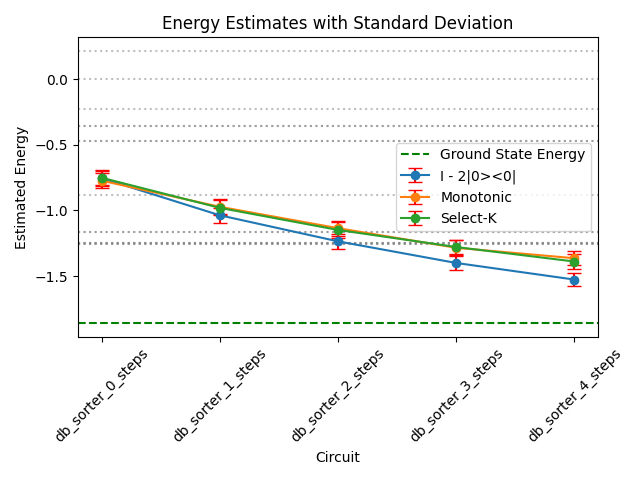
\includegraphics[width=\textwidth]{energy_estimates_H2.png}
        \caption{DB-Sorter run on $H_2$}
        \label{subfig:H2-D-compare}
    \end{subfigure}
    \hfill
    \begin{subfigure}[b]{0.48\textwidth}
        \centering
        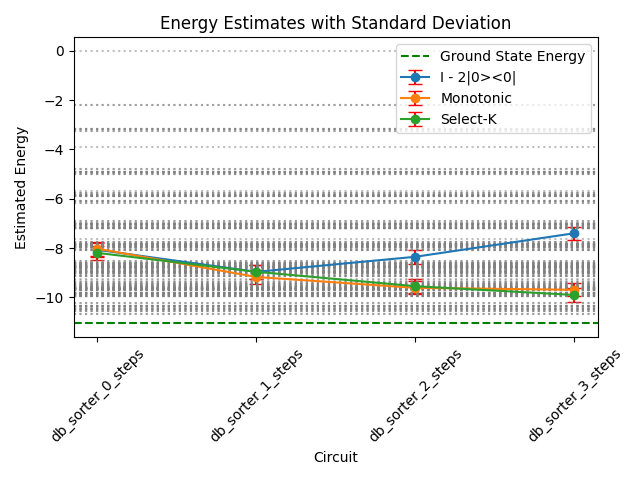
\includegraphics[width=\textwidth]{energy_estimates_NH3.png}
        \caption{DB-Sorter run on $NH_3$}
        \label{subfig:NH3-D-compare}
    \end{subfigure}
    
    % === MAIN CAPTION ===
    \caption{$I - 2\ket{0}\bra{0}$ has a fast convergence but it also introduces more error, while Select-K method in larger Hamiltonians and further steps, marginally outperforms the monotone $D$. In theory, this win would be bigger for even larger hamiltonians or for more steps.}
    \label{fig:grid_main}
\end{figure}

\end{document}
